\documentclass[11pt]{beamer}
\usepackage[UTF8]{ctex}
\usepackage[utf8]{inputenc}
\usepackage[T1]{fontenc}
\usepackage{lmodern}
\usepackage{amsmath}
\usepackage{amsfonts}
\usepackage{amssymb}
\usepackage{graphicx}
\usetheme{CambridgeUS}

\usepackage{pdfpages}


%%%%%
\usepackage{longtable}
\usepackage{subfigure}
\usepackage{color}
\usepackage{booktabs}

%%%%%
\usepackage[backend=bibtex,sorting=none]{biblatex}
\addbibresource{reference.bib} %BibTeX数据文件及位置
\setbeamerfont{footnote}{size=\tiny} 
\setbeamertemplate{bibliography item}[text]

%% LOGO放右上
\setbeamertemplate{frametitle}
{\begin{beamercolorbox}[wd=\paperwidth]{frametitle}
		\strut\hspace{0.5em}\insertframetitle\strut
		\hfill
		\raisebox{-2mm}{
\includegraphics[width=1cm]{figures/HNUC.jpeg}}
	\end{beamercolorbox}
}

%%% 课件属性定义
\author{郭泰彪}
\title{区块链原理及应用}
\subtitle{第6课:区块链分布式系统基础-拜占庭将军问题}
\institute[湖工商大数据研究院]{湖南工商大学大数据与互联网创新研究院}
\date{2020年10月15日}
\titlegraphic{
\includegraphics[width=2cm]{figures/HNUC.jpeg}}

\begin{document}
\begin{frame}	
	\maketitle
\end{frame}

\begin{frame}
	\frametitle{目录}
	\tableofcontents[sectionstyle=show,subsectionstyle=show/shaded]
\end{frame}

\section{导言:生活中的信任}
\subsection{信任方式的变迁}

\begin{frame}{社会现象背后的信任断层}
	内容...
\end{frame}

\begin{frame}{中国传统的血缘信任}
	内容...
\end{frame}

\begin{frame}{西方现代社会的制度化信任}
	内容...
\end{frame}

\begin{frame}{信任的定义}

\end{frame}

\subsection{两种典型的信任模式}

\subsubsection{基于记忆的信任模式}

\subsubsection{通过可信第三方的信任模式}

\section{陌生人间建立信任的问题}
\subsection{陌生人间建立信任}

\subsection{问题推广:不可信机器间建立信任的问题}
\begin{frame}{问题推广:不可信机器间建立信任的问题}
	一个可靠的计算机系统必须能够应付一个或多个组件发生故障。一个失败的组件可能会表现出一种经常被忽视的行为,向系统的不同部分发送冲突的信息。
\end{frame}

\begin{frame}{几个名词的辨析的区别}
	分布式系统的故障:进程或通信通道偏离被认为是正确或期望的行为。
	\begin{enumerate}
		\item 进程故障: 
		\item 通信故障:
		\end{enumerate}
	
	\begin{enumerate}
		\item 进程故障: 
		\item 通信故障:
	\end{enumerate}
\end{frame}

\begin{frame}{利用分布式系统来解决可靠性的例子}
	\begin{figure}
		\centering
		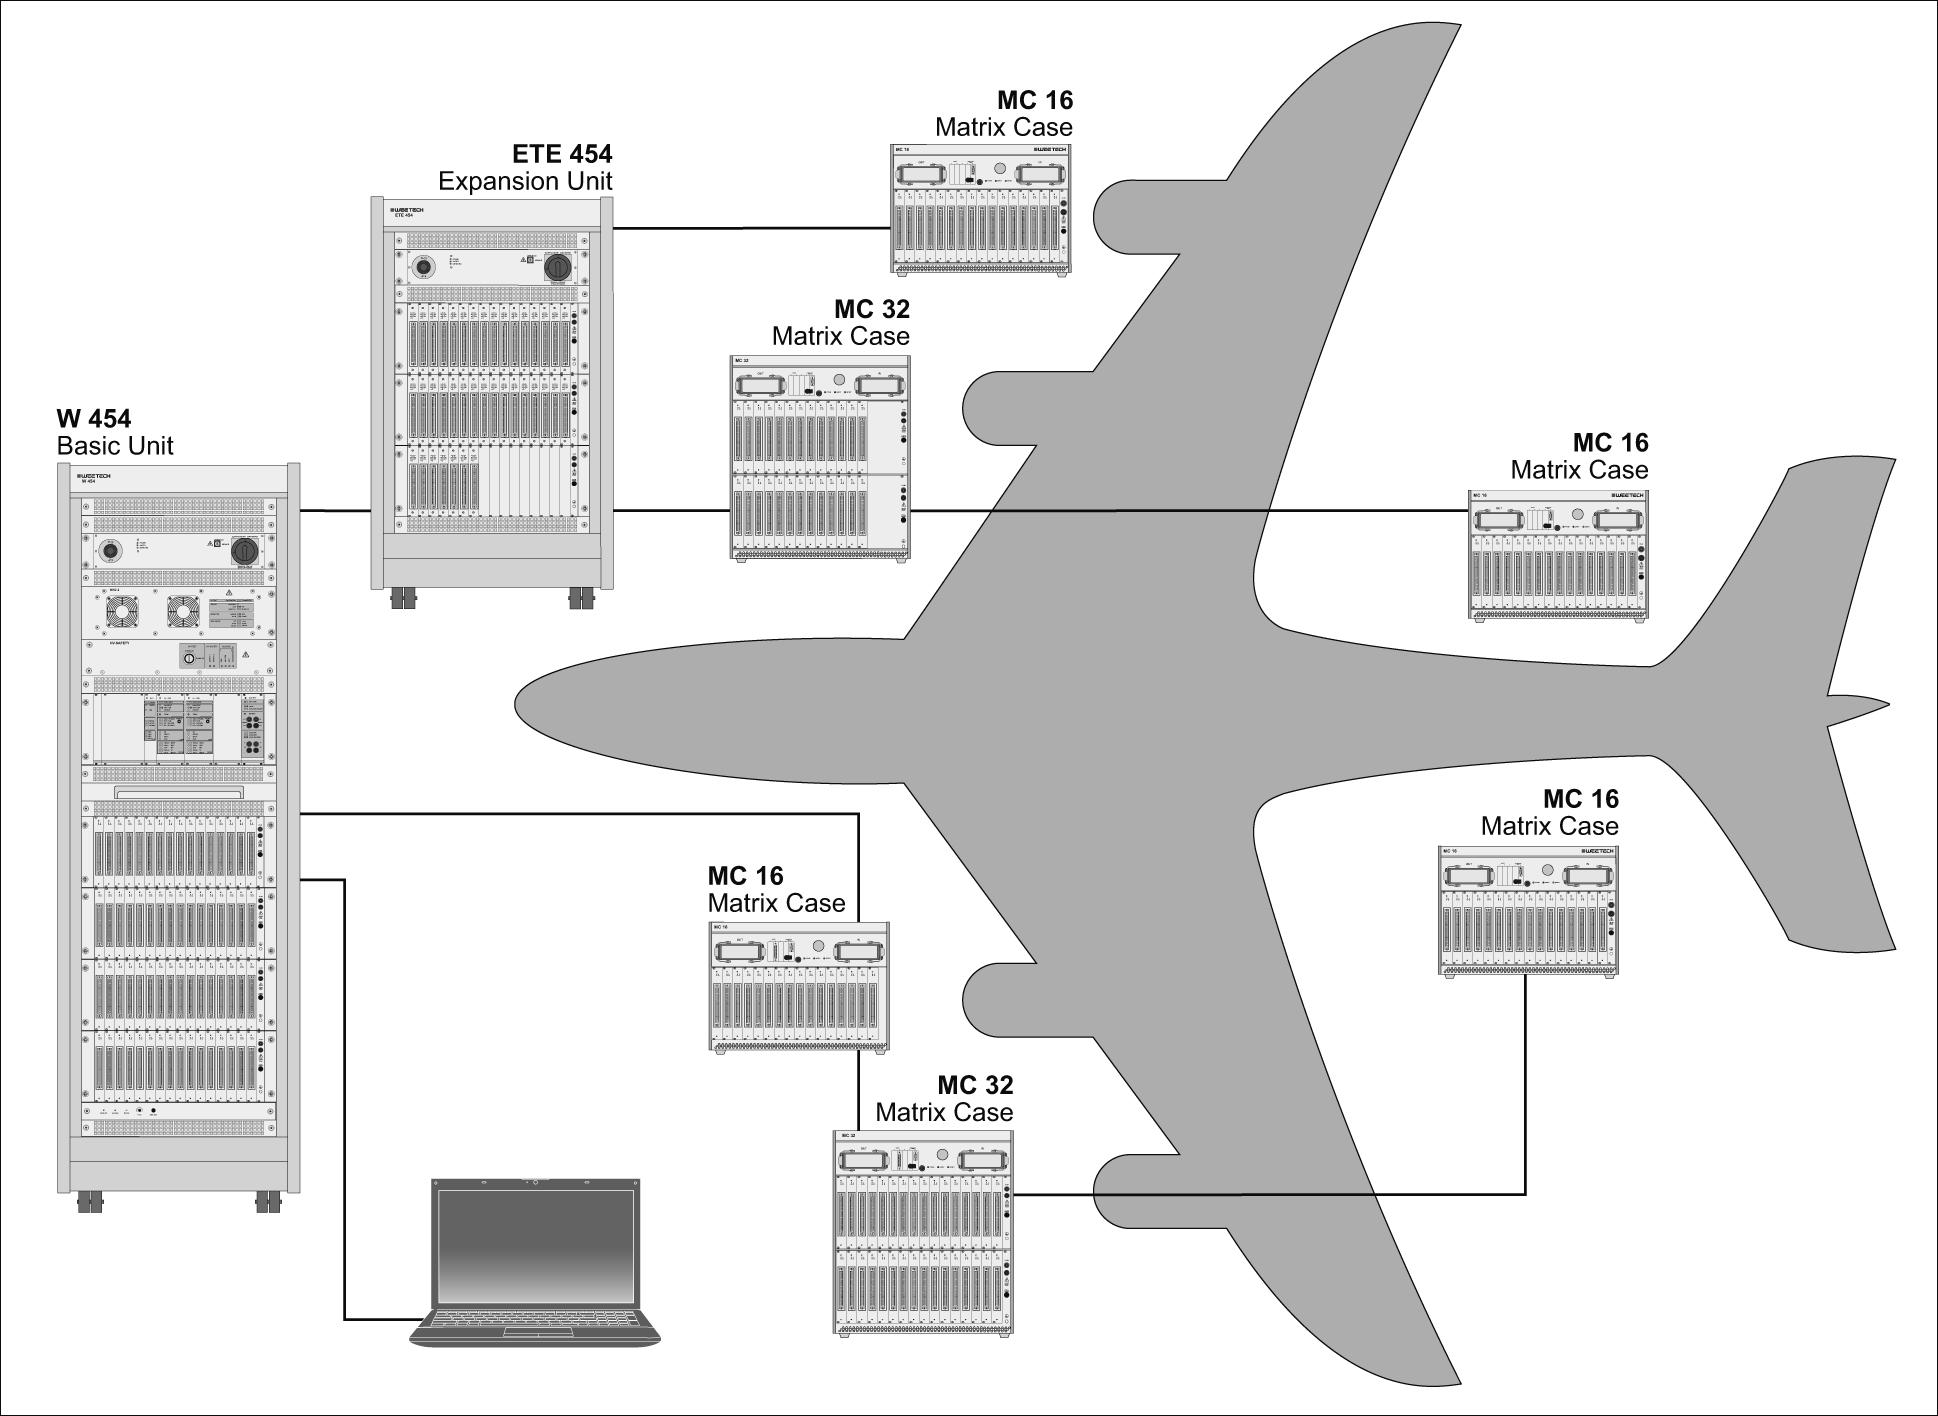
\includegraphics[width=0.7\linewidth]{figures/distributedPlane}
		\caption{飞机利用分布式系统来确保机载计算机系统可靠性}
		\label{fig:distributedplane}
	\end{figure}
	
\end{frame}

% 在网络中存在恶意者的情况下完成程序的执行
\subsection{问题的抽象化:拜占庭将军问题}

\begin{frame}{拜占庭将军问题背景}
	处理这类失败的问题被抽象地表述为拜占庭将军问题\cite{lamport_byzantine_1982}。
	\begin{enumerate}
\item Important to have reliable computer systems
\item  Two solutions to ensuring a reliable system
\begin{enumerate}
\item Having components that never fail
\item Ensure proper handling of cases where components fail
\end{enumerate}
\item Byzantine Generals Problem
	\end{enumerate}
\end{frame}

\begin{frame}{Problem}
\begin{enumerate}
	\item Divisions of the Byzantine army camped outside the walls of an enemy city.
\item  Each division is led by a general.
\item Generals decide on a common plan of action.
\end{enumerate}
\end{frame}

\begin{frame}{Types of Generals}
		There are two types of generals
	\begin{enumerate}
		\item Loyal Generals
		\item Traitor Generals
	\end{enumerate}
\end{frame}

\begin{frame}{Problem – Conditions}
两个条件必须被满足:
\begin{enumerate}
	\item A.所有的忠将都将达成一致的作战计划;
	\item B.少数叛将将无法导致忠将采纳不良计划; 
\end{enumerate}
	\end{frame}

\begin{frame}{Problem - Not a Bad Plan}
作战计划的制定方式:
\begin{enumerate}
	\item 每个将军都将自己侦查的敌方情况发送给其他将军;其中:
	
	\item $v(i)$是第$i$位将军传达的消息,将军总数为$n$;
	
	\item 每位将军通过某种方法将$v(1),...,v(n)$的值结合起来形成一个作战计划;
\end{enumerate}
\end{frame}


\begin{frame}{Problem – Example Not a Bad Plan
}
	\begin{enumerate}
		\item 内容...
	\end{enumerate}
\end{frame}


\begin{frame}{Problem – Example Not a Bad Plan
}
	\begin{enumerate}
		\item General 2 receives ATTACK, ATTACK.
		\item General 3 receives ATTACK, ATTACK.
	\end{enumerate}
So Not a Bad Plan is to ATTACK
\end{frame}

\begin{frame}{Problem – Not a Bad Plan Flaw
}
	\begin{enumerate}
		\item Assumed that every general communicates the same v(i) to every other general.
		\item A traitor general can send different v(i) messages to different generals.
	\end{enumerate}
\end{frame}

\begin{frame}{Problem – Example Flaw}
	\begin{enumerate}
		\item General 2 receives ATTACK, ATTACK.
		\item General 3 receives RETREAT, ATTACK.
	\end{enumerate}
Is Not a Bad Plan to ATTACK or RETREAT?

\end{frame}

\begin{frame}{Problem – New Conditions}
	The new conditions are:
	\begin{enumerate}
		\item Any two loyal generals use the same value of v(i). 
		\item If the $i^{th}$ general is loyal, then the value that he sends must be used by every loyal general as the value of v(i). 
	\end{enumerate}
\end{frame}

\begin{frame}{Byzantine Generals Problem}
	A commander general giving orders to his lieutenant generals.

\textbf{Byzantine Generals Problem} – A commanding general must send an order to his n-1 lieutenant generals such that:
	\begin{enumerate}
		\item {\color{red} IC1}. All loyal lieutenants obey the same order.
		\item {\color{red}IC2}. If the commanding general is loyal, then every loyal lieutenant obeys the order he sends.
	\end{enumerate}
These are called \textbf{the interactive consistency} conditions.
\end{frame}

\begin{frame}{Impossibility Results}
	\begin{enumerate}
		\item When will the Byzantine Generals Problem fail?
		\item The problem will fail if 1/3 or more of the generals are traitors.
	\end{enumerate}
\end{frame}

\begin{frame}{Impossibility Results – Example}
	\begin{enumerate}
		\item L1 received the commands ATTACK, RETREAT
		\item L1 doesn’t know which general is a traitor.
	\end{enumerate}
\end{frame}

\begin{frame}{Impossibility Results – Example 2}
	\begin{enumerate}
		\item L1 again received the commands ATTACK, RETREAT
		\item L1 doesn’t know which general is a traitor.
	\end{enumerate}
\end{frame}

\begin{frame}{Impossibility Results Generalization}
	No solution when:
	\begin{enumerate}
		\item Fewer than {\color{red}3m + 1} generals;
	\end{enumerate}
{\color{red}m} = number of traitor generals
\end{frame}

\begin{frame}{Impossibility Results - Application}
	\begin{enumerate}
		\item Utilized in clock synchronization as described in Dolev et al. [1986] 
		\item N > 3f
		\begin{enumerate}
			\item N = number of clocks
			\item f = number of clocks that are faulty
		\end{enumerate}
		\item Same as the Byzantine Problem!
	\end{enumerate}
\end{frame}

\begin{frame}{Impossibility Results}
	\begin{enumerate}
		\item When will the Byzantine Generals Problem fail?
		\item The problem will fail if 1/3 or more of the generals are traitors.
	\end{enumerate}
\end{frame}

\begin{frame}{Impossibility Results – Example}
	\begin{enumerate}
		\item L1 received the commands ATTACK, RETREAT
		\item L1 doesn’t know which general is a traitor.
	\end{enumerate}
\end{frame}

\begin{frame}{Impossibility Results – Example 2}
	\begin{enumerate}
		\item L1 again received the commands ATTACK, RETREAT
		\item L1 doesn’t know which general is a traitor.
	\end{enumerate}
\end{frame}

\begin{frame}{Impossibility Results Generalization}
	No solution when:
	\begin{enumerate}
		\item Fewer than 3m + 1 generals;
	\end{enumerate}
m = number of traitor generals
\end{frame}

\begin{frame}{Impossibility Results - Application}
	
\end{frame}






\section{区块链:“虚拟”可信第三方}

\subsection{区块链:“虚拟”可信第三方}

\subsection{区块链如何解决陌生人信任问题}

\subsection{问题分解}

\section*{参考文献}
\begin{frame}{参考文献}
	\printbibliography
\end{frame}

\section*{谢谢聆听}

\begin{frame}
	\begin{minipage}[t]{0.5\linewidth}
		\begin{center}
			\begin{figure}
				\vspace{10pt}
				
				{\Huge 谢谢聆听}
				
				\vspace{30pt}
				郭泰彪
				
				\vspace{10pt}
				{\tiny 湖南工商大学大数据与互联网创新研究院}
			\end{figure}
			\begin{figure}
				
			\end{figure}
		\end{center}
	\end{minipage}%
	\begin{minipage}[t]{0.4\linewidth}
		\begin{figure}
			\centering
			\texttt{blockchain101}
			
			
\includegraphics[width=0.6\linewidth]{figures/blockchain101qrcode}
			
			{\footnotesize \texttt{Star| Fork| Issue}}
		\end{figure}
	\end{minipage}%
\end{frame}

\end{document}